\documentclass{article}

% if you need to pass options to natbib, use, e.g.:
% \PassOptionsToPackage{numbers, compress}{natbib}
% before loading nips_2018

% ready for submission
% \usepackage{nips_2018}

% to compile a preprint version, e.g., for submission to arXiv, add
% add the [preprint] option:
% \usepackage[preprint]{nips_2018}

% to compile a camera-ready version, add the [final] option, e.g.:
\usepackage[final]{nips_2018}

% to avoid loading the natbib package, add option nonatbib:
% \usepackage[nonatbib]{nips_2018}

\usepackage[utf8]{inputenc} % allow utf-8 input
\usepackage[T1]{fontenc}    % use 8-bit T1 fonts
\usepackage{hyperref}       % hyperlinks
\usepackage{url}            % simple URL typesetting
\usepackage{booktabs}       % professional-quality tables
\usepackage{amsfonts}       % blackboard math symbols
\usepackage{nicefrac}       % compact symbols for 1/2, etc.
\usepackage{microtype}      % microtypography
\usepackage{graphicx}
\usepackage{float, subcaption}

\title{Summer2Monsoon: Using CycleGAN for Image-to-Image Translation} 

% The \author macro works with any number of authors. There are two
% commands used to separate the names and addresses of multiple
% authors: \And and \AND.
%
% Using \And between authors leaves it to LaTeX to determine where to
% break the lines. Using \AND forces a line break at that point. So,
% if LaTeX puts 3 of 4 authors names on the first line, and the last
% on the second line, try using \AND instead of \And before the third
% author name.

\author{
  Arnav Garg \\
  Department of Computer Science\\
  UCLA\\
  \texttt{arnavgarg@cs.ucla.edu} \\
  \And
  Simranjit Singh \\
  Department of Computer Science\\
  UCLA\\
  \texttt{simranjit@cs.ucla.edu} \\
   \And
  Tanmay Sardesai \\
  Department of Computer Science\\
  UCLA\\
  \texttt{tanmays@cs.ucla.edu} \\
}

\begin{document}
% \nipsfinalcopy is no longer used

\maketitle

\begin{abstract}
 


\end{abstract}

\section{Introduction}

In the past couple of years, there has been a lot of research done on cross domain image to image translation, where an image is taken from one domain and then transformed into an image of the target domain. This is particularly important as a large number of Computer Vision and Machine Learning problems can viewed as an image-to-image translation problem. For example, noise reduction can be considered a mapping between a noisy image to a corresponding noise free image. For many tasks, it is either very difficult or impossible to find paired data, and so in-order to find a mapping between different domains of images, an un-supervised setting is required. The goal of unsupervised image to image translation is to learn the mapping of special characteristics of one image collection and finding how these characteristics could be translated into the other image collection, all in the absence of any paired training examples.

In this paper, we  perform image-to-image translation using cycle-consistent adversarial network, also known as CycleGAN,  to translate a summer scene into a rainy one and visa versa. We also perform single image de-raining. Some of the applications of this include, helping the film industry shoot movies irrespective of the seasonal cycle and helping self-driving car researchers in data collection by transforming summer images to rainy images, which would allow them to train their models on both these environments simultaneously thereby decreasing the time needed for data collection and training.

%We propose a novel method of translating frames/images of environments 
%taken in the summer season to the monsoon season and back. 
%This would allow the data collected by researchers during 
%summer to transform into monsoon conditions and train their 
%models on both these environments simultaneously thereby 
%decreasing the time needed for data collection and training.

%To solve this, we plan to use CycleGAN, which performs image to image 
%translation, by learning the mapping between input image and output image 
%using a training set of unpaired image pairs [1]. CycleGAN captures the 
%special characteristics of one domain and finds out how these 
%characteristics could be translated into the other domain, all in the 
%absence of any paired training examples. In our research, one image 
%collection would be of images taken in during the summer season and 
%the other during the monsoon season. We will discuss this is in greater 
%detail in Section \ref{headings}.  

Some of the other applications of our research include solving the problem of de-raining. There has been various research 
 done on de-raining, as discussed in Section \ref{relatedworks} and we believe that our proposed model would be able to solve the problem by training it to transform rainy images to summer.


% \begin{figure}[htb!]
%  \centering
%  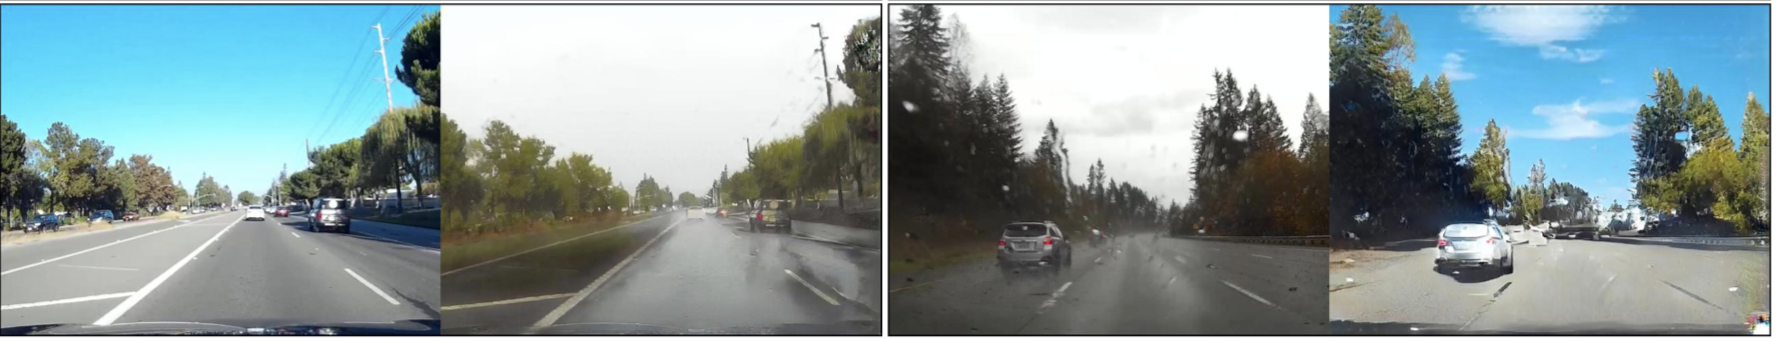
\includegraphics[width=99mm]{image.png}
%  \caption{Taken from nvidia paper. Goal of this project is to do better
%  than this using cycle gan \label{overflow}}
%\end{figure}


\section{Related Work}
\label{relatedworks}

\textbf{Generative Adversarial Networks (GANs)} [2] were introduced by  Ian Goodfellow in 2014 and have been very successful in image-to-image translations. GANs have one neural network that generates data while the other discriminates between real and fake (generated) data. Over time both networks get better at their tasks and the generator is now able to mimic the distribution of the input domain. GAN was used for a variety of applications and it has paved a way for series of GAN-family implementations for different applications.

\textbf{Image-to-Image translation} is the core of this project. The work that we will be exploring in this paper is CycleGAN [1]. Given two domains, $X$ and $Y$, and two generators $G: X \rightarrow Y$ and $F: Y \rightarrow  X$ then we try to achieve a cycle-consistency such that $F(G(X)) \approx X$ and $G(F(Y)) \approx Y$. There is also other work done in the domain of image-to-image translation. The authors of CycleGAN previously proposed pix2pix [5] which used Conditional GANs. pix2pix also has multiple applications but one of the constraints is that pix2pix needs paired data for training. This is sometimes impossible or a really difficult task. For example in our case we would need images taken from the same exact location in 2 different seasons for our dataset. Some related work on image-to-image translation is also done by Nvidia using coupled GAN [3]. Concurrent to the work done in CycleGAN, Yi et al [6], published a paper on dual-GAN.

\textbf{Single Image de-raining} is a difficult problem to solve due to its ill-posed nature and unlike video based methods, images do not provide any temporal information. Traditionally it has been approached as considering an image y to be the sum of rain streak r and background image x, i.e. $y = x + r$. This is why most of the research approaches try to decompose the image into a background image and rain streak image. One of the earliest methods is sparse coding based [a] where image is decomposed using learned dictionary atoms that can sparsely represent two components clearly. Gaussian mixture models based priors [c] have also been used in image decomposition frameworks that can capture different orientations and scales of rain streaks. CNNs have also been employed to directly learn non linear mapping between synthesized images and ground truths successfully for image de-raining [d] [e] [f]. Conditional GANs are also used to achieve de-raining [4]. The work in this, and other papers on de-raining, doesn’t completely solve the problem as they only remove rain from the image but some aspects of the image still look the same as the sky will still look cloudy and the roads will look wet even after removing the rain. These models only work on monsoon to summer translations but not vice versa.

\section{Implementation}
\label{implementation}

\subsection{CycleGAN and training setup}

As mentioned before we use CycleGAN, which performs image to image  translation, by learning the mapping between input image and output image using a training set of unpaired image pairs. CycleGAN captures the special characteristics of one domain and finds out how these characteristics could be translated into the other domain, all in the absence of any paired training examples.

For this project we will train the PyTorch implementation of cycleGAN that is publicly available on GitHub. Our dataset consists of 2 sets of images: summer images and rainy images. There is no one-to-one correspondence between the two sets. Since cycleGAN assumes some underlying relationship between the images from two sets, our first attempt will be to obtain images of the same dataset for two seasons and divide them into train and test datasets. We will show in the next few subsections how we approached this problem.

For training our models we used n1-highmem-2 (2 vCPUS, 13 GB memory) google compute engine. We also had one NVIDIA Tesla K80.

\subsection{Attempt 1}

For our first attempt, we used sunny and rainy images from \textit{Camera as Weather Sensor: Estimating Weather Information from Single Images} [7]. This model didn't work as well as expected. On further inspection we saw some evidence of overfitting. For example as shown in \ref{fig:v1_failure} one can see 2 people in sky of the fake image. We attributed this to bad training data as the data didn't truly represent the real world. One of the reasons why we saw this was because the dataset is classified as sunny or rain based on an estimation that is computed using geotags and by crawling the web for weather properties. 

\begin{figure}[H]
	\begin{subfigure}{.5\textwidth}
		\centering
		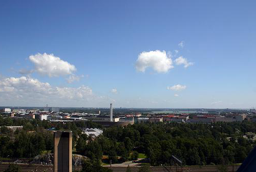
\includegraphics[width=.9\linewidth]{images/v1_real_A.png}
		\caption{Real sunny image}
	\end{subfigure}
	\begin{subfigure}{.5\textwidth}
		\centering
		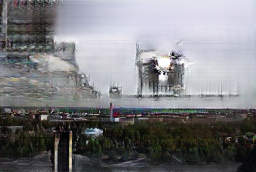
\includegraphics[width=.9\linewidth]{images/v1_fake_B.png}
		\caption{Fake rainy image}
	\end{subfigure}
	\caption{Example of overfitting during the first training}
	\label{fig:v1_failure}
\end{figure}

\subsection{Attempt 2}

Due to the failures from our first attempt we decided to focus on a dataset which had similar images while still depicting the real world distribution. This is why we used images from \textit{Oxford Robotcar Dataset}[8]. 

\subsection{Attempt 3}

[9]


\subsection{De-raining}

[10]


\section{Results}

We performed two different types of studies to help evaluate our results. For our image to image translation, we performed a perceptual study where we created a survey and asked participants to classify if images were real or fake and for the Single Image De-raining, as we had ground truth for these images, we computed the Structural Similarity Index Scores (SSIM) between to de-rained images and the ground-truth to evaluate how well our model performed. We have discussed both of these studies on in the subsection below.

\subsection{Perceptual Study}

\begin{table} [h!]
\centering
\begin{tabular}{ | c | c | c | c |}
\hline
 Type & Total & Real & Fake \\ 
\hline
 Survey 1 (Sunny) &  0.591 & 0.825 & 0.543 \\  
 Survey 2 (Rainy) & 0.597 & 0.716 & 0.578 \\
 \hline
\end{tabular}
\caption{Survey Results}
\label{table:1}
\end{table}

For evaluating our image to image translation model, we conducted two online surveys, one with only summer images and the other with rainy images, in which we showed multiple fake (our model generated) and real images to the participant. In both the surveys, the participants were shown each image for 2 seconds, and then were asked to identify if the image they saw was fake or real. The results of the surveys are shown in table \ref{table:1}. In Survey 1, containing only fake and real summer images, we collected data from 35 participants and for Survey 2, containing only fake and real rainy images, we collected data from 20 participants. The ratio of fake to real images in both these surveys was 24 to 5. 

From Table \ref{table:1} we can see that for the Survey 1, only 59.1\% of the participants were able to correctly guess if the image was real or fake and for Survey 2, only 59.7\% of the people were able to a guess correctly. It is interesting to note that out of all the fake images in our survey, only 54.3\% and 57.8\% of the participants in Survey 1 and  Survey 2 respectively were able to correctly classify that our model generated image was fake, which is impressive compared to other researches done in this area. Although, as the number of participants in both the surveys are very low, the result from this empirical data may or may not be close to the true result. We aim to continue our evaluation and collect more data to have a more accurate result in the future.

\subsection{Structural Similarity Index (SSIM)}


% TODO: Put figure here. 


To evaluate our image-to-image model for de-raining, we compared our model generated de-rained image to the ground truth value and the results presented by Fu et al, in their research paper \textit{"Clearing the Skies: A deep network architecture for single-image rain removal"} as shown in Figure ??. 

\begin{table} [h!]
\centering
\begin{tabular}{ | c | c | c | c | c |}
\hline
 Image & Ground Truth & Paper (Fu et. al) & Ours & Rainy Image \\ 
\hline
 Umbrella & 1 & 0.88 & 0.83 & 0.80 \\
 Rabbit & 1 & 0.85 & 0.765 & 0.767 \\
 Bird & 1 & 0.82 & 0.702 & 0.55 \\
 100 images (avg) & 1 & 0.89 & 0.80 & 0.62 \\
 \hline
\end{tabular}
\caption{SSIM Scores}
\label{table:2}
\end{table}

Table \ref{table:2} shows the SSIM scores for the ground truth, Fu et. al model, our model and the noisy image. It can be seen that our model performed comparable to Fu et. al model however wasn't able to beat their accuracy. Our understanding is that our model fell short because our training dataset contained rain noise that were only vertical strokes of rain. When we tested our model on Fu et. al's testing dataset, which contained diagonal rain strokes, our model couldn't outperform their model. Due to time constraints we weren't able to generate our desired dataset and train our model again. For our future work, we plan on training our model again with a more diverse training dataset, to see if it helps improve our accuracy and outperform Fu et. al's mode. 

It also surprising to see that the SSIM score for the rain image of the bird was lower than the SSIM score of our model generated de-rained image and we plan on looking further into why that might be the case as part of our future work. 

\section{Limitation \& Discussions}

TODO

\section{Conclusion \& Future Work}

We have employed the CycleGAN model for the purpose of translating images from summer to monsoon and vice-versa. We were successfully able to train the model to minimize the proposed loss function on our final dataset collected from various sources. We conducted a survey to see if users can identify fake images as real and achieved results comparable to what is discussed in CycleGAN paper. We also employed CycleGAN to de-rain the images as well as add rain to images and evaluated the results based on SSIM scores and compared to some of the previous works.

In future, we want to explore the model used in [3] that involves shared latent space and believe that it would give better results than our current model. In our model the generator loss did not converge but overall loss did and that is something we are keen on analyzing. The loss proposed in CycleGAN is weighted sum of different losses and we believe that these weights can be tuned to achieve even better results.

\section*{References}

\small
\label{[1]}[1] J. Zhu, T. Park, P. Isola, and A. A. Efros. Unpaired image-to-image 
translation using cycle-consistent adversarial networks. 
In International Conference on Computer Vision (ICCV), to appear, 2017

\label{[2]}[2] I. Goodfellow, J. Pouget-Abadie, M. Mirza, B. Xu, D. Warde-Farley, 
S. Ozair, A. Courville, and Y. Ben- gio. Generative adversarial nets. 
In NIPS, 2014.

\label{[3]}[3] M.-Y. Liu, T. Breuel, and J. Kautz. Unsupervised 
image-to-image translation networks. arXiv preprint arXiv:1703.00848, 2017

\label{[4]}[4] H. Zhang, V. A. Sindagi, and V. M. Patel. Image de-raining using a conditional generative 
adversarial network. arXiv preprint arXiv:1701.05957, 2017.

\label{[5]}[5] P. Isola, J.-Y. Zhu, T. Zhou, and A. A. Efros. 
Image-to-image translation with conditional adversarial networks. 
In CVPR, 2017

\label{[6]}[6] Z. Yi, H. Zhang, T. Gong, Tan, and M. Gong. Dualgan: 
Unsupervised dual learning for image-to-image translation. 
In ICCV, 2017

\label{[7]}[7] Wei-Ta Chu, Xiang-You Zheng, and Ding-Shiuan Ding, "Camera as Weather Sensor: Estimating Weather Information from Single Images," Journal of Visual Communications and Image Representation, vol. 46, pp. 233-249, 2017.

\label{[8]}[8] W. Maddern, G. Pascoe, C. Linegar and P. Newman, "1 Year, 1000km: The Oxford RobotCar Dataset", The International Journal of Robotics Research (IJRR), 2016.

\label{[9]}[9] Amato, Giuseppe and Carrara, Fabio and Falchi, Fabrizio and Gennaro, Claudio and Meghini, Carlo and Vairo, Claudio, "Deep learning for decentralized parking lot occupancy detection". Expert Systems with Applications, vol 72, pp. 327-334, 2017

\label{[10]}[10] X. Fu, J. Huang, X. Ding, Y. Liao, and J. Paisley, “Clearing the Skies: A deep network architecture for single-image rain removal,” ArXiv eprints, Sep. 2016.

\end{document}
